\documentclass{standalone}

\usepackage{times}
\usepackage{amsmath}
\usepackage{amssymb}

\usepackage[dvipsnames]{xcolor}
\usepackage{tikz}
\usepackage{tikz-qtree}
\usetikzlibrary{arrows,backgrounds,scopes}

\usepackage{pgfplots}
\pgfplotsset{compat=1.15}
\begin{document}
	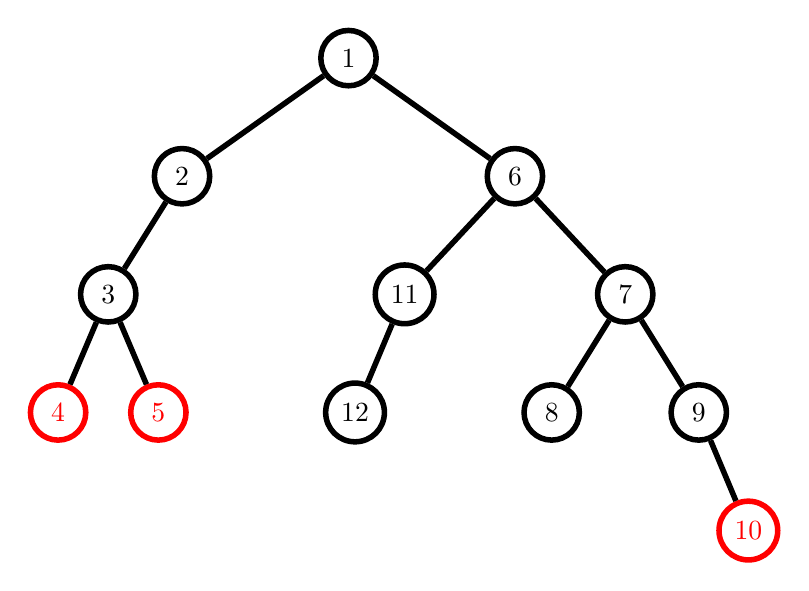
\begin{tikzpicture}[every tree node/.style={minimum width=2em,draw,circle,line width=2pt,},
		blank/.style={draw=none},
		edge from parent/.style=
		{draw, line width=2pt, edge from parent path={(\tikzparentnode) -- (\tikzchildnode)}},
		level distance=1.5cm,
		sibling distance=0.5cm,
		marked/.style={color=red}]
		\Tree
		[.1     
			[.2
				[.3 
					\edge; \node[marked]{4};
					\edge; \node[marked]{5};
				]
				\edge[blank]; \node[blank]{};
			]
			[.6 
				[.11 
					[.12 ]
					\edge[blank]; \node[blank]{};
				]
				[.7 
					[.8 ]
					[.9 
						\edge[blank]; \node[blank]{};
						\edge; \node[marked]{10};
					]
				]
			]
		]
	\end{tikzpicture}
\end{document} 
